\section{Pruebas}
\label{sec:pruebas}

La validación del modelo se realizó ejecutando casos de prueba en el
intérprete de la VDM++ Toolbox. Los casos cubren las operaciones de
búsqueda y combinan resultados esperados positivos y negativos, usando
las coordenadas de la Plaza de Armas como origen y del Terminal
Terrestre como destino. La Tabla~\ref{tab:pruebas} resume los casos
ejecutados.

\begin{table}[!t]
\centering
\caption{Casos de prueba ejecutados en el intérprete.}
\label{tab:pruebas}
\small
\begin{tabular}{|c|p{4.1cm}|p{2.1cm}|}
\hline
Caso & Entrada & Resultado \\
\hline
P1 & Origen y destino sobre el recorrido, radio 0.05 & Devuelve la ruta \\
\hline
N1 & Origen lejano, radio 0.05 & Conjunto vacío \\
\hline
C1 & Dos recorridos con transbordo & Par de rutas \\
\hline
\end{tabular}
\end{table}

En el caso positivo, el recorrido contiene puntos exactamente en el
origen y en el destino, por lo que la distancia mínima es nula y el
recorrido se devuelve. En el caso negativo se utiliza un origen lejano,
de modo que ningún recorrido cumple la restricción de distancia y el
resultado es el conjunto vacío. En el caso combinado, dos recorridos
comparten un punto de transbordo dentro del radio establecido.

La Figura~\ref{fig:pruebas} muestra la ejecución de estos casos en el
intérprete, con los recorridos construidos como tuplas y el sentido como
valor \emph{quote} (\texttt{<IDA>}).

\begin{figure}[!t]
\centering
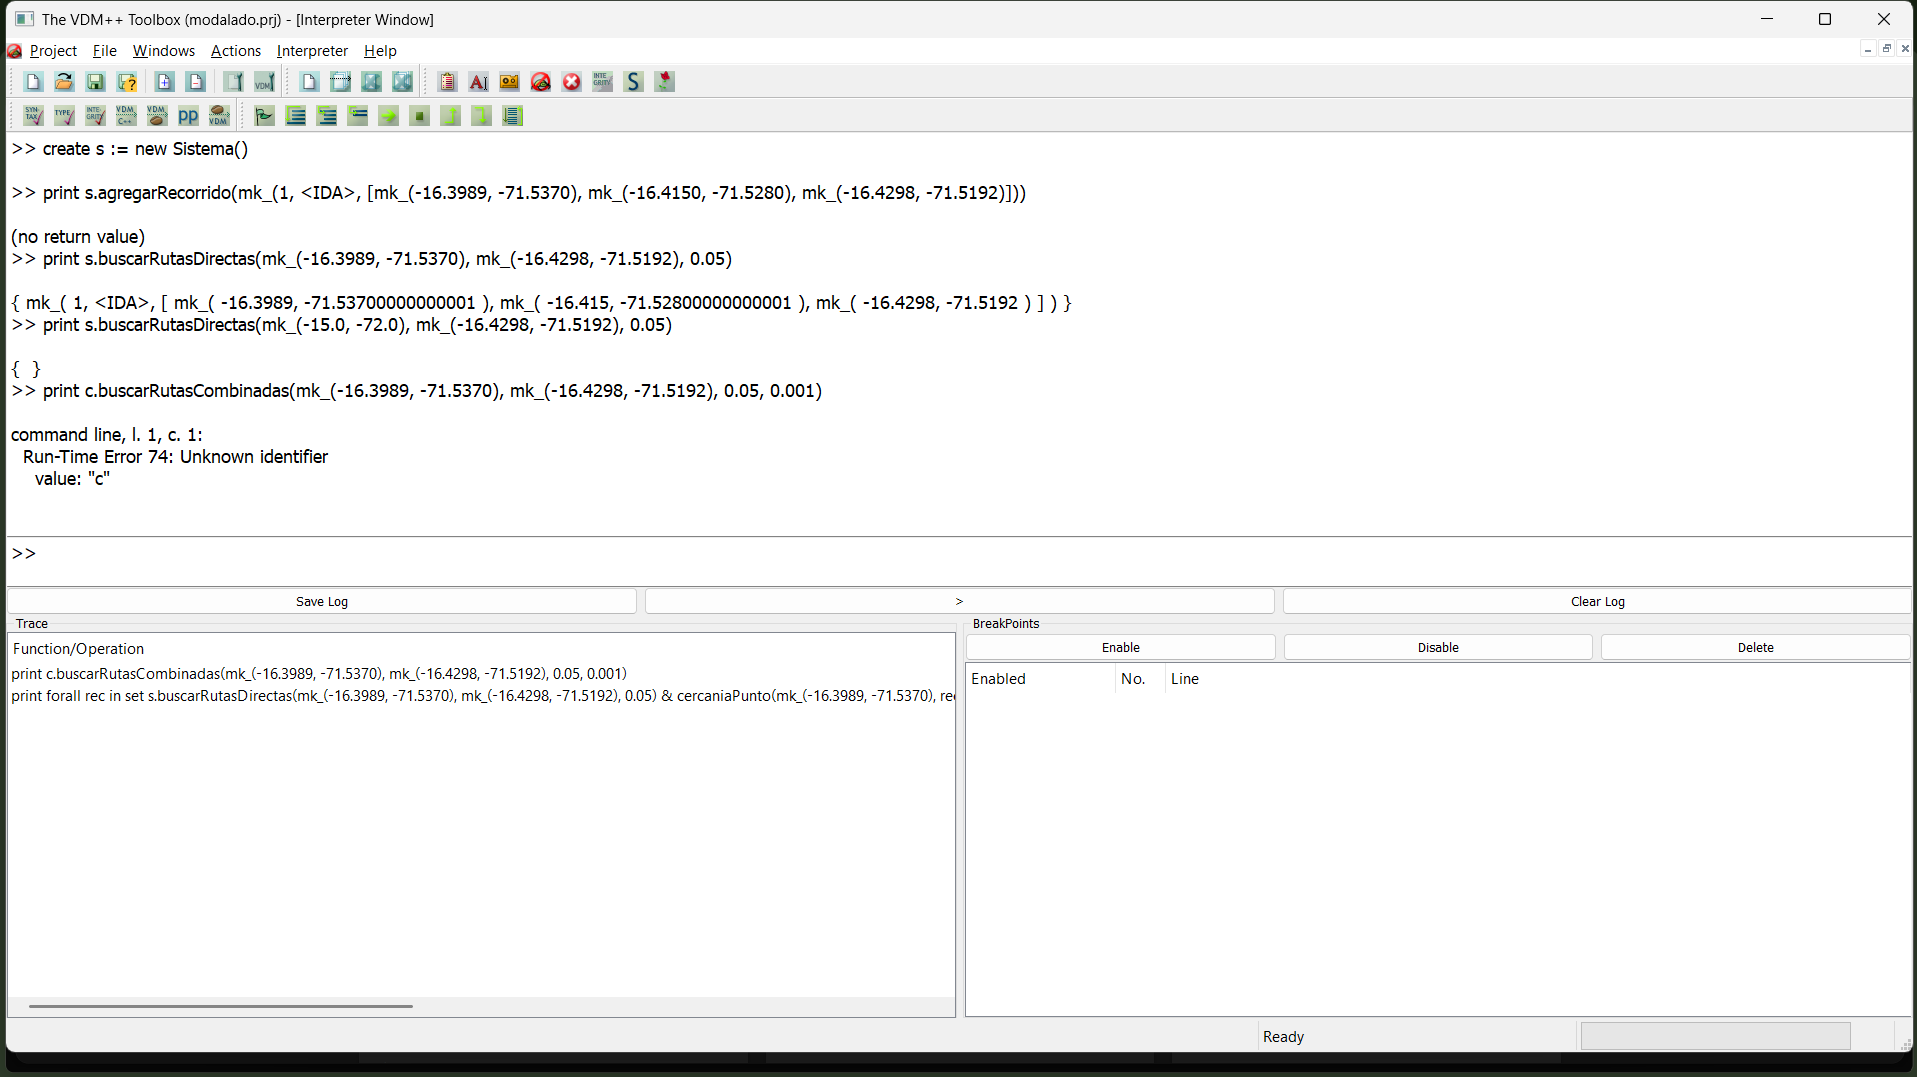
\includegraphics[width=\columnwidth]{images/Casos_de_Prueba.png}
\caption{Ejecución de los casos de prueba en el intérprete de la Toolbox.}
\label{fig:pruebas}
\end{figure}
